\documentclass[11pt,a4paper]{article}

% ========== PACKAGES ==========
\usepackage[utf8]{inputenc}
\usepackage[T1]{fontenc}
\usepackage[french]{babel}
\usepackage{amsmath,amssymb,amsthm}
\usepackage{graphicx}
\usepackage{algorithm}
\usepackage{algorithmic}
\usepackage{tikz}
\usepackage{pgfplots}
\pgfplotsset{compat=1.18}
\usetikzlibrary{shapes,arrows,positioning,calc,decorations.pathreplacing}
\usepackage{hyperref}
\usepackage{geometry}
\usepackage{booktabs}
\usepackage{listings}
\usepackage{xcolor}

\geometry{margin=2.5cm}
\emergencystretch=1em

% ========== ENVIRONNEMENTS THÉORIQUES ==========
\newtheorem{definition}{Définition}[section]
\newtheorem{proposition}[definition]{Proposition}
\newtheorem{theoreme}[definition]{Théorème}
\newtheorem{remarque}[definition]{Remarque}

% ========== STYLE CODE ==========
\lstset{
    language=Python,
    basicstyle=\ttfamily\scriptsize,
    keywordstyle=\color{blue}\bfseries,
    commentstyle=\color{green!60!black}\itshape,
    stringstyle=\color{red!70!black},
    showstringspaces=false,
    breaklines=true,
    frame=single,
    backgroundcolor=\color{gray!10},
    numbers=left,
    numberstyle=\tiny\color{gray}
}

% ========== TITRE ==========
\title{L'algorithme HDBSCAN : Fondements Mathématiques et Implémentation\\ Rapport de recherche en apprentissage automatique}
\author{ZAMANILEHA Elorgin Fernando et RANDRIAMAMONJY Tokiniaina}
\date{13 octobre 2025}

\begin{document}

\maketitle

\begin{abstract}
Ce rapport présente une analyse mathématique rigoureuse de l'algorithme HDBSCAN (Hierarchical Density-Based Spatial Clustering of Applications with Noise). Nous détaillons les fondements théoriques de cette méthode de clustering, incluant la transformation des distances par atteignabilité mutuelle, la construction de l'arbre couvrant minimum, et l'extraction des clusters par l'algorithme GAP. L'implémentation pas à pas est présentée avec un code Python commenté. Cette étude s'adresse aux étudiants et chercheurs en mathématiques appliquées et informatique souhaitant comprendre en profondeur les mécanismes algorithmiques d'HDBSCAN.
\end{abstract}

\tableofcontents

\section{Introduction}

\subsection{Le clustering : définition et enjeux}

Le clustering constitue l'une des tâches fondamentales de l'apprentissage non supervisé. Étant donné un ensemble de $n$ points de données $X = \{x_1, x_2, \ldots, x_n\}$ dans un espace métrique, l'objectif du clustering est de partitionner ces points en groupes (clusters) tels que les points au sein d'un même groupe soient similaires, tandis que les points de groupes distincts présentent une dissimilarité marquée. Cette problématique trouve des applications dans de nombreux domaines : segmentation d'image, analyse de données biologiques, détection d'anomalies, et bien d'autres.

Formellement, on recherche une partition $\mathcal{C} = \{C_1, C_2, \ldots, C_k\}$ de $X$ maximisant une fonction objectif intra-cluster (cohésion) tout en minimisant une fonction objectif inter-cluster (séparation). La difficulté réside dans le fait que le nombre de clusters $k$ est généralement inconnu, et que la notion de « similarité » dépend fortement du contexte applicatif.

\subsection{Clustering basé sur la densité}

Les méthodes de clustering basées sur la densité reposent sur l'intuition suivante : un cluster est une région de l'espace où la densité de points est élevée, séparée d'autres clusters par des régions de faible densité. Cette approche présente plusieurs avantages significatifs par rapport aux méthodes centroides (comme K-means) : elle permet de détecter des clusters de forme arbitraire (non nécessairement convexes), elle identifie naturellement les points aberrants comme du bruit, et elle ne requiert pas la spécification a priori du nombre de clusters.

Le précurseur de cette famille d'algorithmes est DBSCAN (Density-Based Spatial Clustering of Applications with Noise), introduit par Ester et al. en 1996. DBSCAN définit la notion de \textit{core point} (point central) : un point $p$ est central s'il possède au moins $\mathit{minPts}$ points dans son voisinage $\epsilon$. Les clusters sont alors construits en connectant les points centraux entre eux lorsque leur distance mutuelle est inférieure à $\epsilon$.

\subsection{Limitations de DBSCAN}

Malgré son succès, DBSCAN souffre de limitations importantes que nous détaillons ci-dessous :

\textbf{Sensibilité au paramètre $\epsilon$} : Le choix de $\epsilon$ est critique. Une valeur trop petite fragmente les clusters, tandis qu'une valeur trop grande fusionne des clusters distincts. Il n'existe pas de méthode universelle pour déterminer $\epsilon$ de manière optimale.

\textbf{Incapacité à gérer des densités variables} : DBSCAN utilise un seuil de densité global, ce qui le rend inadapté aux données présentant des clusters de densités hétérogènes. Un cluster dense et un cluster diffus ne peuvent être détectés simultanément avec un même paramétrage.

\textbf{Absence de hiérarchie} : DBSCAN produit une partition unique, ne permettant pas d'explorer la structure multi-échelle des données. Or, cette information hiérarchique est souvent précieuse pour l'analyse exploratoire.

\subsection{Motivation pour HDBSCAN}

HDBSCAN (Hierarchical DBSCAN), développé par Campello et al. en 2013, adresse ces limitations en combinant les avantages du clustering basé sur la densité avec le clustering hiérarchique. Les innovations clés d'HDBSCAN sont les suivantes :

Premièrement, l'introduction de la \textit{distance d'atteignabilité mutuelle} transforme l'espace des données de manière à rendre les clusters de densités variables comparables. Cette transformation permet de traiter simultanément des clusters de densités différentes sans paramétrage spécifique.

Deuxièmement, l'utilisation de l'\textit{arbre couvrant minimum} comme structure de données fondamentale permet une construction efficace de la hiérarchie des clusters. Le MST capture les connexions les plus « naturelles » entre les points selon la métrique transformée.

Troisièmement, la notion de \textit{stabilité des clusters} permet une extraction automatique des clusters les plus pertinents, éliminant le besoin de spécifier un seuil de coupe manuel.

\subsection{Vue d'ensemble de l'algorithme}

L'algorithme HDBSCAN peut être décomposé en six étapes principales que nous détaillerons dans les sections suivantes :

\begin{enumerate}
    \item Calcul des \textit{core distances} pour chaque point
    \item Transformation des distances par \textit{mutual reachability}
    \item Construction du graphe d'atteignabilité mutuelle
    \item Calcul de l'arbre couvrant minimum (MST)
    \item Construction de la hiérarchie (dendrogramme)
    \item Condensation et extraction des clusters stables
\end{enumerate}

\section{Fondements mathématiques}

\subsection{Espace métrique et fonction distance}

\begin{definition}[Espace métrique]
Un espace métrique est un couple $(E, d)$ où $E$ est un ensemble et $d : E \times E \to \mathbb{R}_+$ est une fonction vérifiant les propriétés suivantes pour tout $x, y, z \in E$ :
\begin{enumerate}
    \item \textbf{Non-négativité} : $d(x, y) \geq 0$
    \item \textbf{Identité des indiscernables} : $d(x, y) = 0 \Leftrightarrow x = y$
    \item \textbf{Symétrie} : $d(x, y) = d(y, x)$
    \item \textbf{Inégalité triangulaire} : $d(x, z) \leq d(x, y) + d(y, z)$
\end{enumerate}
\end{definition}

Dans le contexte du clustering, nous travaillons généralement avec des points dans $\mathbb{R}^m$ muni de la distance euclidienne :
\begin{equation}
d(x, y) = \sqrt{\sum_{i=1}^{m} (x_i - y_i)^2} = \|x - y\|_2
\end{equation}

\subsection{k-plus proches voisins}

\begin{definition}[$k$-voisin le plus proche]
Soit $X = \{x_1, \ldots, x_n\}$ un ensemble de points et $x_i \in X$. On note $N_k(x_i)$ l'ensemble des $k$ plus proches voisins de $x_i$ dans $X \setminus \{x_i\}$, défini par :
\begin{equation}
N_k(x_i) = \arg\min_{S \subseteq X \setminus \{x_i\}, |S| = k} \max_{x_j \in S} d(x_i, x_j)
\end{equation}
\end{definition}

Intuitivement, $N_k(x_i)$ contient les $k$ points les plus proches de $x_i$ (en excluant $x_i$ lui-même). La taille de ce voisinage est un indicateur local de la densité : dans une région dense, le $k$-voisin le plus proche est proche, tandis que dans une région sparse, il est plus éloigné.

\subsection{Core distance}

\begin{definition}[Core distance]
La \textit{core distance} d'un point $x_i$ par rapport au paramètre $k$ est définie comme la distance au $k$-ième plus proche voisin :
\begin{equation}
\boxed{\text{core}_k(x_i) = d(x_i, x^{(k)}_i)}
\end{equation}
où $x^{(k)}_i$ désigne le $k$-ième plus proche voisin de $x_i$.
\end{definition}

La core distance est une mesure locale de densité inverse. Un point dans une région de haute densité aura une petite core distance, tandis qu'un point isolé aura une grande core distance. Formellement, on peut établir la relation suivante avec l'estimateur de densité par noyau :

\begin{proposition}
La core distance $\text{core}_k(x)$ est inversement proportionnelle à la racine $m$-ième de la densité locale $\rho(x)$ dans un espace de dimension $m$ :
\begin{equation}
\text{core}_k(x) \propto \rho(x)^{-1/m}
\end{equation}
\end{proposition}

\begin{proof}[Esquisse de preuve]
Dans une région de densité $\rho$, le nombre attendu de points dans une boule de rayon $r$ est $n \cdot \rho \cdot V_m r^m$, où $V_m$ est le volume de la boule unité en dimension $m$. En posant ce nombre égal à $k$, on obtient $r \propto \rho^{-1/m}$.
\end{proof}

\subsection{Distance d'atteignabilité mutuelle}

\begin{definition}[Mutual reachability distance]
La \textit{distance d'atteignabilité mutuelle} entre deux points $x_i$ et $x_j$ est définie par :
\begin{equation}
\boxed{d_{\text{mreach}}(x_i, x_j) = \max\bigl\{\text{core}_k(x_i), \text{core}_k(x_j), d(x_i, x_j)\bigr\}}
\end{equation}
\end{definition}

Cette transformation de distance est l'innovation clé d'HDBSCAN. Elle présente plusieurs propriétés fondamentales qui justifient son utilisation.

\begin{proposition}
La distance d'atteignabilité mutuelle $d_{\text{mreach}}$ est une métrique sur l'ensemble des points.
\end{proposition}

\begin{proof}
Vérifions les quatre propriétés :
\begin{enumerate}
    \item \textbf{Non-négativité} : Immédiat car $\max$ de termes non-négatifs.
    \item \textbf{Identité} : $d_{\text{mreach}}(x, x) = \max\{\text{core}_k(x), \text{core}_k(x), 0\} = \text{core}_k(x) > 0$ pour $x$ non isolé. Notez que ce n'est pas exactement $0$, mais cette propriété ne pose pas de problème pour le clustering.
    \item \textbf{Symétrie} : $d_{\text{mreach}}(x_i, x_j) = d_{\text{mreach}}(x_j, x_i)$ par symétrie de $\max$ et de $d$.
    \item \textbf{Inégalité triangulaire} : Pour tout $x_i, x_j, x_l$, on a :
    \begin{align}
    d_{\text{mreach}}(x_i, x_l) &= \max\{\text{core}_k(x_i), \text{core}_k(x_l), d(x_i, x_l)\} \\
    &\leq \max\{\text{core}_k(x_i), \text{core}_k(x_l), d(x_i, x_j) + d(x_j, x_l)\} \\
    &\leq \max\{\text{core}_k(x_i), \text{core}_k(x_j), d(x_i, x_j)\} \nonumber\\
    &\quad + \max\{\text{core}_k(x_j), \text{core}_k(x_l), d(x_j, x_l)\} \\
    &= d_{\text{mreach}}(x_i, x_j) + d_{\text{mreach}}(x_j, x_l)
    \end{align}
\end{enumerate}
\end{proof}

\begin{figure}[htbp]
\centering
\begin{tikzpicture}[scale=0.9]
    % Points dans cluster dense
    \fill[blue!60] (0,0) circle (3pt) node[below left] {$x_i$};
    \fill[blue!60] (0.8,0.3) circle (3pt);
    \fill[blue!60] (0.3,0.7) circle (3pt);
    \fill[blue!60] (0.5,-0.4) circle (3pt);
    \fill[blue!60] (-0.4,0.5) circle (3pt);
    \draw[blue!40, dashed] (0,0) circle (0.6);
    \node[blue!70] at (0,-1.2) {\small $\text{core}_k(x_i)$ petit};
    
    % Points dans cluster sparse
    \fill[red!60] (5,0) circle (3pt) node[below left] {$x_j$};
    \fill[red!60] (6.5,0.5) circle (3pt);
    \fill[red!60] (6.2,-0.7) circle (3pt);
    \fill[red!60] (4.3,0.8) circle (3pt);
    \fill[red!60] (5.8,1.2) circle (3pt);
    \draw[red!40, dashed] (5,0) circle (1.8);
    \node[red!70] at (5,-1.2) {\small $\text{core}_k(x_j)$ grand};
    
    % Ligne entre les deux points
    \draw[thick, ->] (0.3,0) -- (4.7,0) node[midway, above] {$d(x_i, x_j)$};
    
    % Illustration de la mreach
    \node at (2.5,-2.5) {\small $d_{\text{mreach}}(x_i, x_j) = \max\{\text{core}_k(x_i), \text{core}_k(x_j), d(x_i, x_j)\}$};
\end{tikzpicture}
\caption{Illustration de la distance d'atteignabilité mutuelle entre un point d'un cluster dense et un point d'un cluster diffus.}
\label{fig:mreach}
\end{figure}

\begin{figure}[ht]
\centering
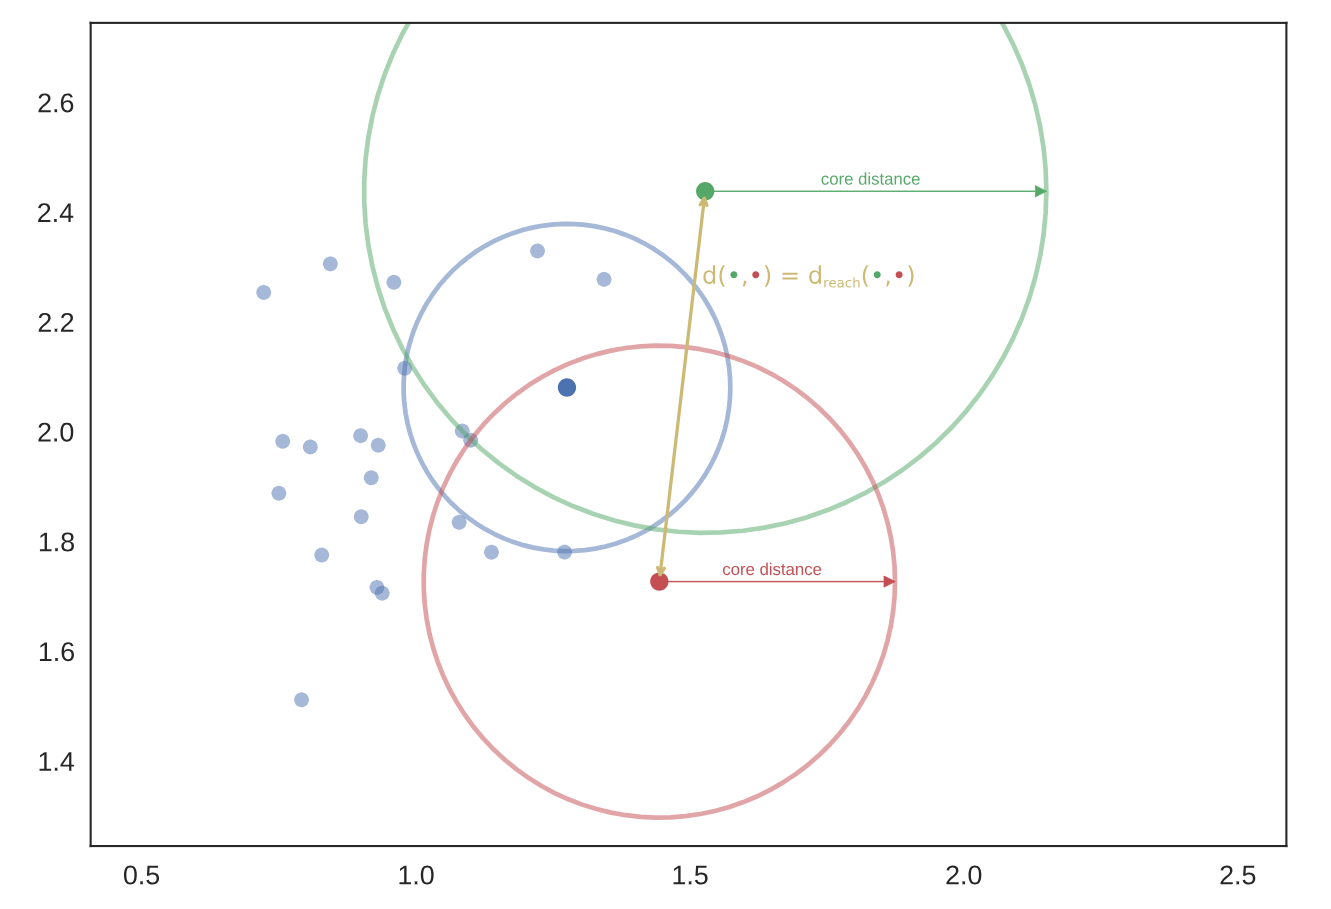
\includegraphics[width=0.6\textwidth]{image/img_3.png}
\caption{Visualisation complémentaire de la distance d'atteignabilité mutuelle sur un exemple de données.}
\label{fig:mreach_img3}
\end{figure}

\begin{remarque}
L'intuition géométrique est la suivante : si deux points sont dans des clusters de densités différentes, la distance d'atteignabilité mutuelle « lisse » cette différence en imposant que traverser une région de basse densité « coûte » plus cher. Cela permet de détecter des clusters de densités variables comme des entités comparables.
\end{remarque}

\section{Construction du graphe d'atteignabilité mutuelle}

\subsection{Représentation graphique des données}

Étant donné un ensemble de $n$ points $X = \{x_1, \ldots, x_n\}$, nous construisons un graphe complet pondéré $G = (V, E, w)$ où :
\begin{itemize}
    \item $V = X$ est l'ensemble des sommets (chaque point est un sommet)
    \item $E = \{(x_i, x_j) : i < j\}$ est l'ensemble des arêtes
    \item $w : E \to \mathbb{R}_+$ attribue à chaque arête le poids $d_{\text{mreach}}(x_i, x_j)$
\end{itemize}

Le graphe complet possède $\binom{n}{2} = \frac{n(n-1)}{2}$ arêtes, ce qui peut devenir prohibitif pour de grands jeux de données. Cependant, la structure particulière du problème permet des optimisations que nous discuterons.

\subsection{Propriétés du graphe d'atteignabilité mutuelle}

\begin{proposition}
Le graphe d'atteignabilité mutuelle possède les propriétés suivantes :
\begin{enumerate}
    \item Il est \textbf{connexe} : il existe un chemin entre toute paire de sommets
    \item Les arêtes de faible poids connectent des points de même densité locale
    \item Les arêtes de fort poids traversent des régions de basse densité ou connectent des clusters distincts
\end{enumerate}
\end{proposition}

Ces propriétés sont fondamentales : elles signifient que les clusters naturels correspondent à des sous-graphes fortement connectés par des arêtes de faible poids, séparés par des arêtes de fort poids.

\begin{figure}[htbp]
\centering
\begin{tikzpicture}[
    scale=0.8,
    node/.style={circle, draw, minimum size=6pt, inner sep=2pt},
    edge weak/.style={thin, blue!60},
    edge strong/.style={thick, red!60}
]
    % Cluster 1 (dense)
    \node[node, fill=blue!30] (a1) at (0,0) {};
    \node[node, fill=blue!30] (a2) at (0.8,0.5) {};
    \node[node, fill=blue!30] (a3) at (0.3,1) {};
    \node[node, fill=blue!30] (a4) at (-0.5,0.6) {};
    
    % Cluster 2 (dense)
    \node[node, fill=green!30] (b1) at (4,0) {};
    \node[node, fill=green!30] (b2) at (4.8,0.5) {};
    \node[node, fill=green!30] (b3) at (4.3,1) {};
    \node[node, fill=green!30] (b4) at (3.5,0.6) {};
    
    % Point de bruit
    \node[node, fill=gray!50] (n) at (2,0) {};
    
    % Arêtes intra-cluster (faible poids)
    \draw[edge weak] (a1) -- (a2) -- (a3) -- (a4) -- (a1);
    \draw[edge weak] (a1) -- (a3) (a2) -- (a4);
    \draw[edge weak] (b1) -- (b2) -- (b3) -- (b4) -- (b1);
    \draw[edge weak] (b1) -- (b3) (b2) -- (b4);
    
    % Arêtes inter-cluster (fort poids)
    \draw[edge strong, dashed] (a2) -- (n);
    \draw[edge strong, dashed] (n) -- (b4);
    
    % Légende
    \node at (2,-1.5) {\small Arêtes bleues = faible poids (intra-cluster)};
    \node at (2,-2) {\small Arêtes rouges = fort poids (inter-cluster)};
\end{tikzpicture}
\caption{Représentation schématique du graphe d'atteignabilité mutuelle avec deux clusters et un point de bruit.}
\label{fig:graph}
\end{figure}

\section{Arbre couvrant minimum}

\subsection{Définitions fondamentales}

\begin{definition}[Arbre couvrant]
Soit $G = (V, E)$ un graphe connexe. Un \textit{arbre couvrant} de $G$ est un sous-graphe $T = (V, E_T)$ avec $E_T \subseteq E$ tel que :
\begin{enumerate}
    \item $T$ est un arbre (acyclique et connexe)
    \item $T$ couvre tous les sommets de $G$
\end{enumerate}
\end{definition}

\begin{definition}[Arbre couvrant minimum]
Soit $G = (V, E, w)$ un graphe pondéré. L'\textit{arbre couvrant minimum} (MST) est un arbre couvrant $T^*$ minimisant la somme des poids des arêtes :
\begin{equation}
T^* = \arg\min_{T \text{ arbre couvrant}} \sum_{e \in E_T} w(e)
\end{equation}
\end{definition}

Le MST est unique si toutes les arêtes ont des poids distincts, ce qui est généralement le cas pour des données continues.

\subsection{Algorithme de Prim}

L'algorithme de Prim construit le MST de manière gloutonne, en partant d'un sommet arbitraire et en ajoutant itérativement l'arête de poids minimal reliant un sommet visité à un sommet non visité.

\begin{algorithm}[htbp]
\caption{Algorithme de Prim pour le MST}
\begin{algorithmic}[1]
\REQUIRE Graphe pondéré $G = (V, E, w)$, $|V| = n$
\ENSURE Arbre couvrant minimum $T$
\STATE $\text{key}[v] \leftarrow \infty$ pour tout $v \in V$
\STATE $\text{parent}[v] \leftarrow \text{nil}$ pour tout $v \in V$
\STATE $\text{visited}[v] \leftarrow \text{faux}$ pour tout $v \in V$
\STATE Choisir un sommet initial $s$; $\text{key}[s] \leftarrow 0$
\FOR{$i = 1$ \TO $n$}
    \STATE $u \leftarrow$ sommet non visité avec $\text{key}[u]$ minimal
    \STATE $\text{visited}[u] \leftarrow \text{vrai}$
    \FOR{chaque sommet $v$ non visité adjacent à $u$}
        \IF{$w(u,v) < \text{key}[v]$}
            \STATE $\text{key}[v] \leftarrow w(u,v)$
            \STATE $\text{parent}[v] \leftarrow u$
        \ENDIF
    \ENDFOR
\ENDFOR
\STATE Construire $T$ à partir des arêtes $(v, \text{parent}[v])$
\RETURN $T$
\end{algorithmic}
\end{algorithm}

\subsection{Analyse de complexité}

La complexité de l'algorithme de Prim dépend de la structure de données utilisée pour trouver le sommet de clé minimale :
\begin{itemize}
    \item Avec un tableau simple : $O(n^2)$
    \item Avec un tas binaire : $O((n + m) \log n)$ où $m = |E|$
    \item Avec un tas de Fibonacci : $O(m + n \log n)$
\end{itemize}

Pour le graphe d'atteignabilité mutuelle qui est complet ($m = n^2/2$), la complexité avec un tas est $O(n^2 \log n)$. Cependant, des implémentations optimisées utilisant les $k$-plus proches voisins peuvent réduire cette complexité.

\subsection{Importance du MST pour HDBSCAN}

\begin{proposition}
Le MST du graphe d'atteignabilité mutuelle encode la hiérarchie complète des clusters.
\end{proposition}

L'intuition est la suivante : en supprimant les $k$ arêtes de plus grand poids du MST, on obtient exactement $k+1$ composantes connexes, correspondant à une partition des données à un certain niveau de la hiérarchie. Les arêtes de fort poids correspondent aux « ponts » entre clusters, tandis que les arêtes de faible poids connectent des points au sein d'un même cluster.

\begin{figure}[htbp]
\centering
\begin{tikzpicture}[scale=0.7]
    % Points
    \foreach \x/\y/\name in {0/0/a, 1/0.5/b, 0.5/1/c, -0.3/0.6/d, 4/0/e, 5/0.5/f, 4.5/1/g, 3.7/0.6/h} {
        \node[circle, fill, inner sep=1.7pt] (\name) at (\x,\y) {};
    }
    
    % Arêtes du MST (intra-cluster)
    \draw[thick, blue] (a) -- (b);
    \draw[thick, blue] (b) -- (c);
    \draw[thick, blue] (a) -- (d);
    \draw[thick, blue] (d) -- (c);
    \draw[thick, blue] (e) -- (f);
    \draw[thick, blue] (f) -- (g);
    \draw[thick, blue] (e) -- (h);
    \draw[thick, blue] (h) -- (g);
    
    % Arête inter-cluster (à couper)
    \draw[thick, red, dashed] (b) -- (e) node[midway, above] {\small poids élevé};
    
    % Labels
    \node at (0.3,-0.8) {\small Cluster 1};
    \node at (4.3,-0.8) {\small Cluster 2};
    \node at (2.5,-2) {\small Coupe de l'arête rouge $\Rightarrow$ 2 clusters};
\end{tikzpicture}
\caption{Arbre couvrant minimum (MST) illustrant la séparation de deux clusters par suppression d'une arête inter-cluster.}
\label{fig:mst_separation_clusters}
\end{figure}

\begin{figure}[htbp]
\centering
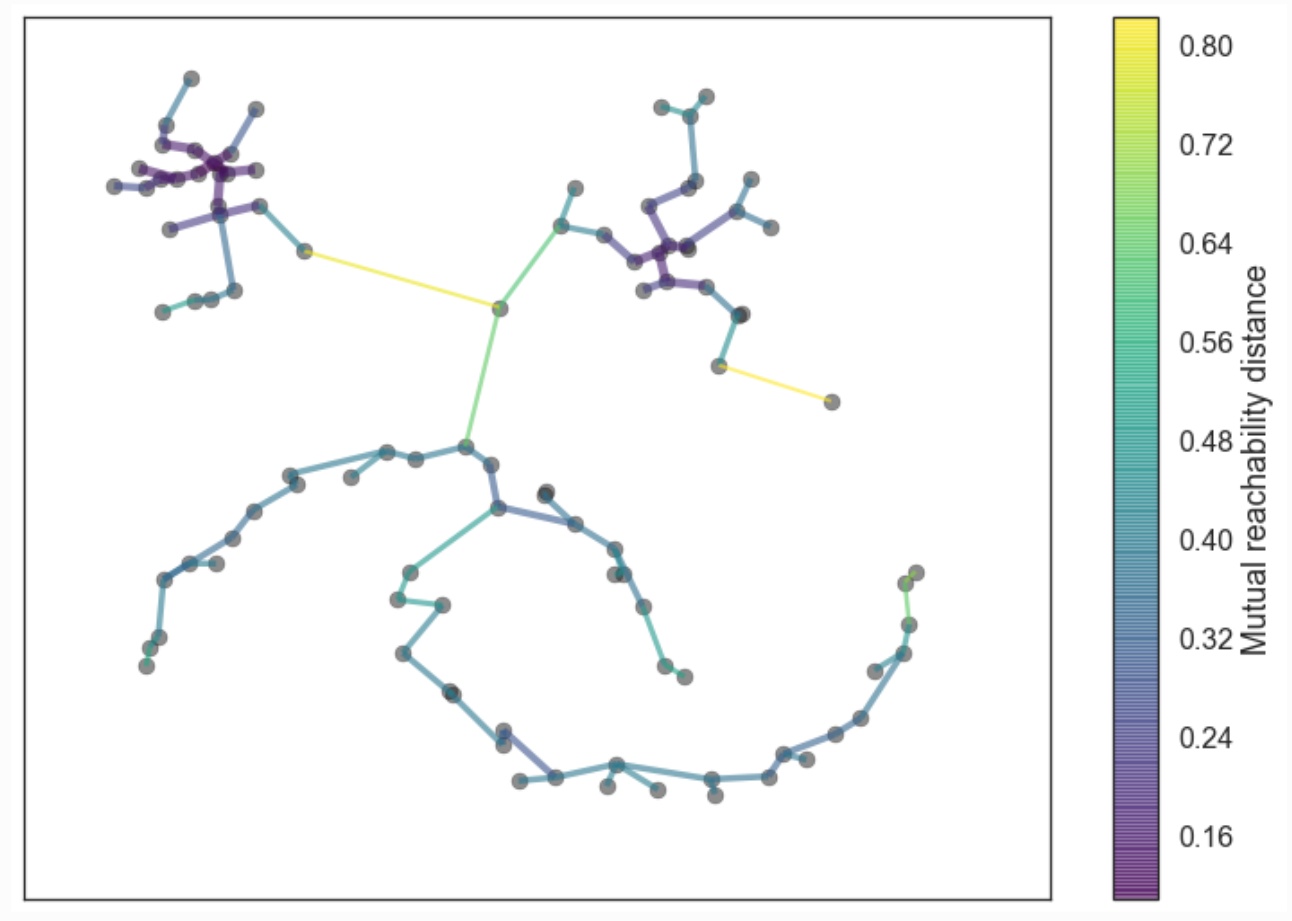
\includegraphics[width=0.6\textwidth]{image/img_5.png}
\caption{Exemple visuel du MST après séparation des clusters (illustration complémentaire).}
\label{fig:mst_separation_complement}
\end{figure}

\section{Clustering hiérarchique et dendrogramme}

\subsection{Construction de la hiérarchie}

Le MST induit naturellement une hiérarchie de clusters. Considérons les arêtes du MST triées par ordre croissant de poids : $e_1, e_2, \ldots, e_{n-1}$. La construction de la hiérarchie procède comme suit :

\begin{enumerate}
    \item Initialement, chaque point forme son propre cluster singleton
    \item À l'étape $t$, on ajoute l'arête $e_t$ qui fusionne deux clusters
    \item Le poids de $e_t$ est la distance de fusion
\end{enumerate}

Cette procédure est identique au clustering hiérarchique agglomératif avec lien simple (single linkage), mais effectué sur la distance d'atteignabilité mutuelle plutôt que la distance euclidienne originale.

\subsection{Dendrogramme}

\begin{definition}[Dendrogramme]
Un \textit{dendrogramme} est une représentation arborescente de la hiérarchie des fusions. Chaque nœud interne représente une fusion, et la hauteur du nœud correspond à la distance de fusion.
\end{definition}

Le dendrogramme permet de visualiser la structure multi-échelle des données. Une coupe horizontale du dendrogramme à une hauteur $\lambda$ produit une partition des données en clusters.

\begin{figure}[htbp]
\centering
\begin{tikzpicture}[scale=0.8]
    % Feuilles (points)
    \foreach \i in {1,...,8} {
        \draw (\i,0) -- (\i,0.5);
        \node at (\i,-0.3) {\tiny $x_{\i}$};
    }
    
    % Fusions
    \draw (1,0.5) -- (1,1) -- (2,1) -- (2,0.5);
    \draw (3,0.5) -- (3,0.8) -- (4,0.8) -- (4,0.5);
    \draw (5,0.5) -- (5,1.2) -- (6,1.2) -- (6,0.5);
    \draw (7,0.5) -- (7,0.6) -- (8,0.6) -- (8,0.5);
    
    % Niveau suivant
    \draw (1.5,1) -- (1.5,1.5) -- (3.5,1.5) -- (3.5,0.8);
    \draw (5.5,1.2) -- (5.5,2) -- (7.5,2) -- (7.5,0.6);
    
    % Fusion finale
    \draw (2.5,1.5) -- (2.5,3) -- (6.5,3) -- (6.5,2);
    
    % Échelle
    \draw[->] (0,0) -- (0,3.5) node[above] {$\lambda$};
    \node at (-0.5,1) {\small $\lambda_1$};
    \node at (-0.5,2) {\small $\lambda_2$};
    \node at (-0.5,3) {\small $\lambda_3$};
    \draw[dashed, gray] (0,1) -- (9,1);
    \draw[dashed, gray] (0,2) -- (9,2);
    \draw[dashed, gray] (0,3) -- (9,3);
\end{tikzpicture}
\caption{Dendrogramme illustrant la hiérarchie des fusions.}
\label{fig:dendrogram}
\end{figure}

\begin{figure}[htbp]
\centering
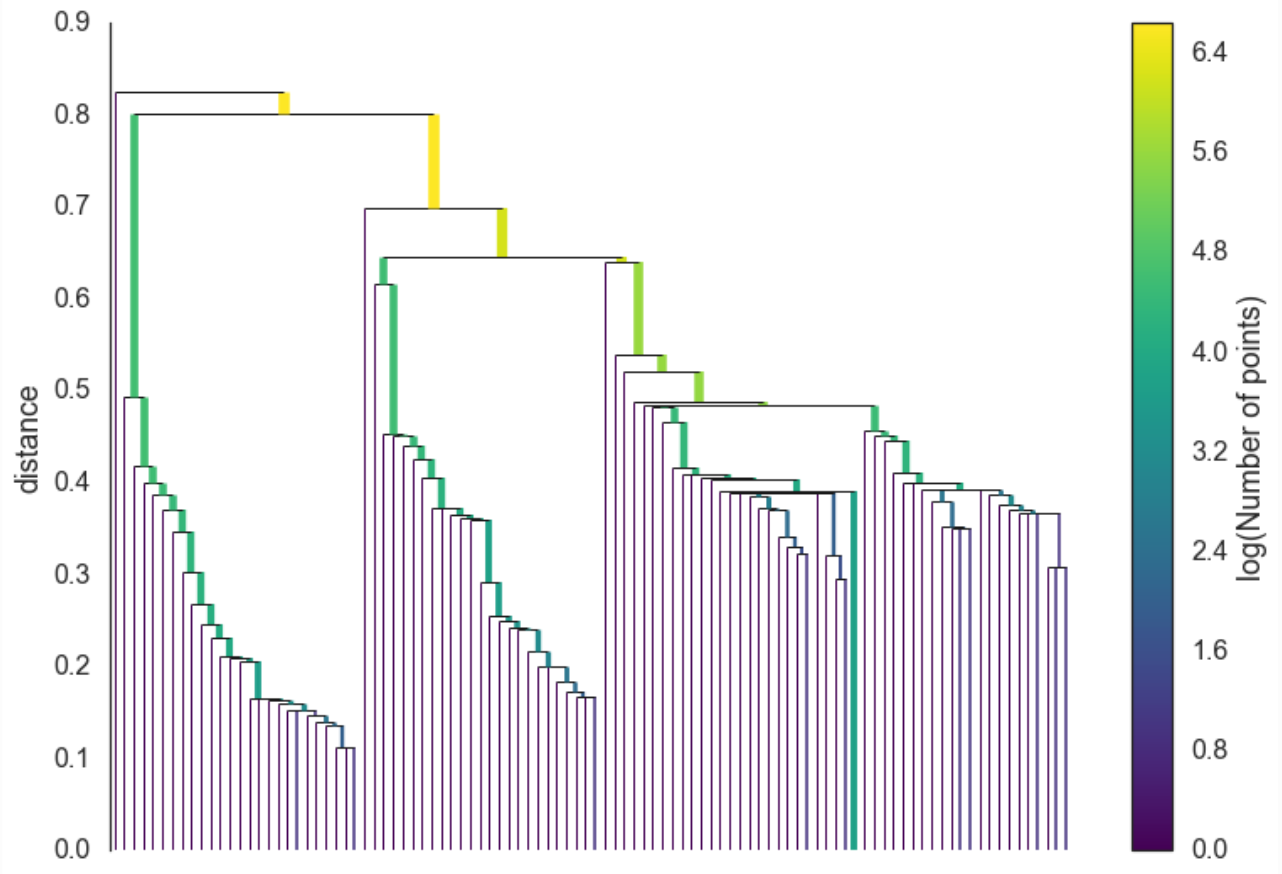
\includegraphics[width=0.6\textwidth]{image/img_4.png}
\caption{Exemple visuel du Dendrogramme illustrant la hiérarchie des fusions (illustration complémentaire).}
\label{fig:dendrogram_img_4}
\end{figure}

\section{Arbre condensé}

\subsection{Motivation}

Le dendrogramme complet contient $n-1$ niveaux, ce qui peut être trop détaillé pour une analyse pratique. L'arbre condensé simplifie cette hiérarchie en ne conservant que les fusions impliquant des clusters de taille suffisante.

\subsection{Paramètre min\_cluster\_size}

\begin{definition}[Taille minimale de cluster]
Le paramètre $\text{min\_cluster\_size}$ (noté $m$) définit le seuil en dessous duquel un groupe de points n'est pas considéré comme un cluster valide.
\end{definition}

Lorsqu'une fusion produit un cluster de taille inférieure à $m$, ce cluster est « absorbé » par son parent et n'apparaît pas comme un nœud séparé dans l'arbre condensé.

\subsection{Processus de condensation}

La condensation s'effectue en parcourant le dendrogramme de bas en haut et en appliquant les règles suivantes :

\begin{enumerate}
    \item Si un cluster a une taille $\geq m$, il est conservé comme nœud dans l'arbre condensé
    \item Si un cluster a une taille $< m$ au moment de la fusion, ses points sont réassignés au cluster parent
    \item La condensation préserve la relation de parenté entre clusters stables
\end{enumerate}

\subsection{Persistance des clusters}

\begin{definition}[Persistance d'un cluster]
La \textit{persistance} d'un cluster $C$ est définie comme la différence entre son niveau de « mort » $\lambda_{\text{death}}$ et son niveau de « naissance » $\lambda_{\text{birth}}$ :
\begin{equation}
\text{persistance}(C) = \lambda_{\text{death}}(C) - \lambda_{\text{birth}}(C)
\end{equation}
\end{definition}

Un cluster persistant survit sur une large plage de valeurs de $\lambda$, ce qui indique qu'il s'agit d'une structure robuste. À l'inverse, un cluster éphémère n'apparaît que pour une plage étroite de $\lambda$.

\section{Extraction des clusters par stabilité}

\subsection{Définition formelle}

\begin{definition}[Stabilité d'un cluster]
La \textit{stabilité} d'un cluster $C$ est définie comme :
\begin{equation}
\boxed{S(C) = \sum_{p \in C} \bigl(\lambda_p - \lambda_{\text{birth}}(C)\bigr)}
\end{equation}
où $\lambda_p = 1/d_{\text{mreach}}(p, \cdot)$ est l'inverse de la distance d'atteignabilité du point $p$ au moment où il quitte le cluster $C$.
\end{definition}

La stabilité mesure la « masse » accumulée par le cluster au cours de son existence. Elle correspond géométriquement à l'aire sous la courbe du profil de densité du cluster.

\subsection{Interprétation géométrique}

Considérons la courbe qui, pour chaque valeur de $\lambda$, indique le nombre de points dans le cluster $C$. La stabilité $S(C)$ est exactement l'aire sous cette courbe. Un cluster stable présente une large base (beaucoup de points sur une grande plage de $\lambda$), tandis qu'un cluster instable a une base étroite.

\begin{figure}[htbp]
\centering
\begin{tikzpicture}[scale=0.9]
    \begin{axis}[
        xlabel={$\lambda = 1/\text{distance}$},
        ylabel={Nombre de points dans $C$},
        xmin=0, xmax=5,
        ymin=0, ymax=50,
        width=10cm,
        height=5cm,
        axis lines=left
    ]
    % Cluster stable (grande aire)
    \addplot[fill=blue!30, draw=blue, thick] coordinates {(0,0) (0,45) (2,45) (4,45) (4,0)} --cycle;
    \node at (axis cs:2,25) {$S(C_1)$};
    
    % Cluster instable (petite aire)
    \addplot[fill=red!30, draw=red, thick, opacity=0.7] coordinates {(4,0) (4,20) (4.5,20) (4.5,0)} --cycle;
    \node at (axis cs:4.25,10) {$S(C_2)$};
    \end{axis}
\end{tikzpicture}
\caption{Interprétation géométrique de la stabilité comme aire sous la courbe.}
\label{fig:stability}
\end{figure}

\begin{figure}[ht]
\centering
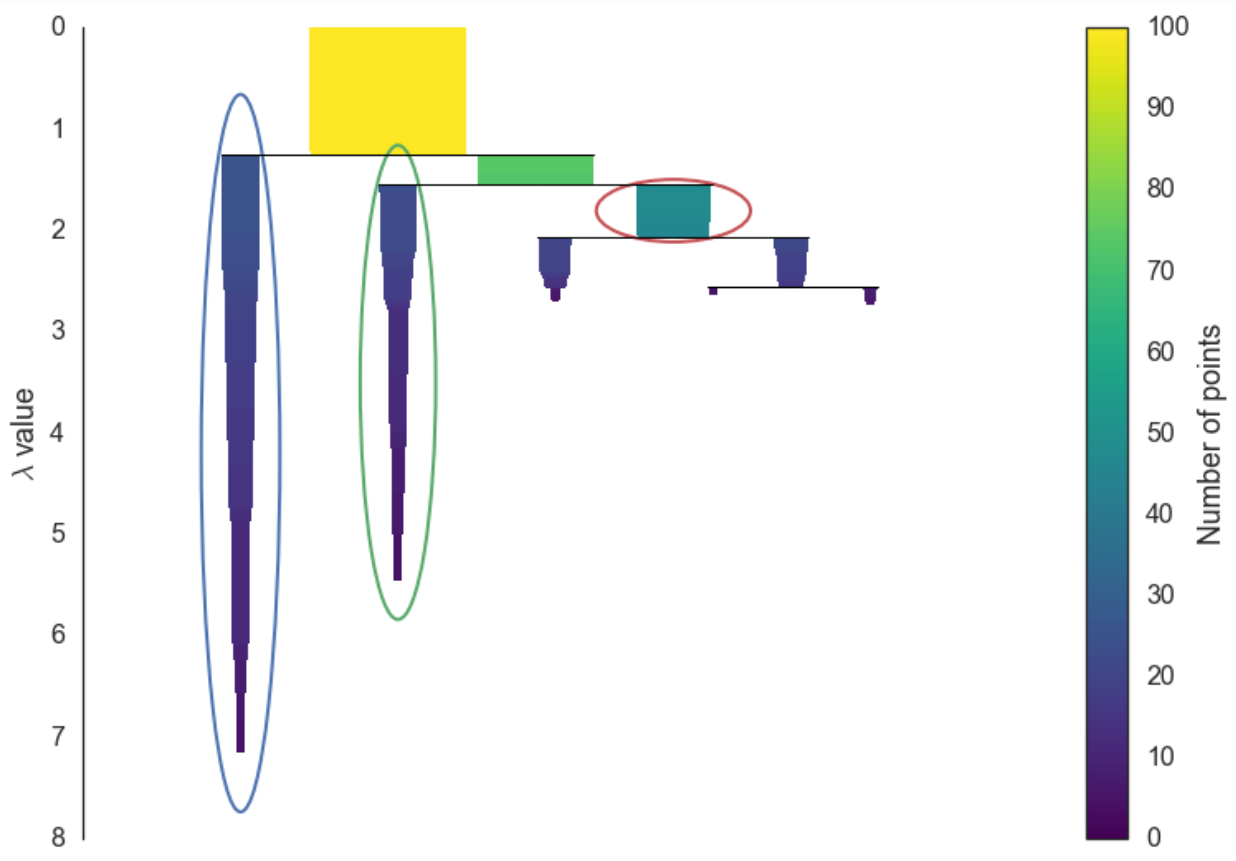
\includegraphics[width=0.5\textwidth]{image/img_6.png}
\caption{Interprétation géométrique de la stabilité comme aire sous la courbe (illustration complémentaire).}
\label{fig:stability_img_6}
\end{figure}

\subsection{Algorithme de sélection}

L'algorithme de sélection des clusters optimaux procède par programmation dynamique sur l'arbre condensé :
\begin{enumerate}
    \item Calculer la stabilité de chaque nœud de l'arbre
    \item Pour chaque nœud, comparer la stabilité du nœud à la somme des stabilités de ses enfants
    \item Si la stabilité du nœud est supérieure, sélectionner le nœud comme cluster final
    \item Sinon, sélectionner récursivement les enfants
\end{enumerate}

Cette approche garantit une sélection optimale au sens de la maximisation de la stabilité totale.

\section{Algorithme GAP pour l'extraction des clusters}

\subsection{Motivation}

L'algorithme GAP (Gap-based Automatic Partitioning) fournit une méthode automatique pour identifier les seuils de coupure naturels dans la hiérarchie. Cette méthode exploite l'observation empirique que les poids des arêtes du MST présentent souvent des « sauts » naturels correspondant aux frontières entre clusters.

\subsection{Formulation mathématique}

Soit $w_1 \leq w_2 \leq \ldots \leq w_{n-1}$ les poids des arêtes du MST triés par ordre croissant. On définit les écarts entre poids consécutifs :
\begin{equation}
g_i = w_{i+1} - w_i, \quad i = 1, \ldots, n-2
\end{equation}

Le principe de l'algorithme GAP est de trouver l'indice du plus grand écart :
\begin{equation}
\boxed{i_{\max} = \arg\max_{i} g_i}
\end{equation}

Le seuil optimal est alors défini comme le point milieu :
\begin{equation}
\boxed{\theta = \frac{w_{i_{\max}} + w_{i_{\max}+1}}{2}}
\end{equation}

\subsection{Justification théorique}

\begin{proposition}
Si les données contiennent $k$ clusters bien séparés, les $k-1$ arêtes de plus fort poids du MST correspondent aux arêtes inter-clusters, tandis que les $n-k$ arêtes de plus faible poids sont intra-clusters.
\end{proposition}

\begin{proof}[Esquisse de preuve]
Les arêtes inter-clusters traversent des régions de basse densité, donc leur distance d'atteignabilité mutuelle est élevée (car la core distance des points de jonction est grande). Les arêtes intra-clusters connectent des points de haute densité, donc leur distance d'atteignabilité est plus faible. Par conséquent, il existe un saut naturel dans la distribution des poids à la frontière entre les arêtes intra et inter-clusters.
\end{proof}

\subsection{Algorithme GAP}

\begin{algorithm}[htbp]
\caption{Algorithme GAP pour la sélection du seuil}
\begin{algorithmic}[1]
\REQUIRE Poids du MST : $w_1 \leq w_2 \leq \ldots \leq w_{n-1}$
\ENSURE Seuil optimal $\theta$ et percentile associé
\STATE Calculer $g_i = w_{i+1} - w_i$ pour $i = 1, \ldots, n-2$
\STATE $i_{\max} \leftarrow \arg\max_i g_i$
\STATE $\theta \leftarrow (w_{i_{\max}} + w_{i_{\max}+1})/2$
\STATE percentile $\leftarrow 100 \cdot i_{\max} / (n-1)$
\RETURN $\theta$, percentile
\end{algorithmic}
\end{algorithm}

\begin{figure}[htbp]
\centering
\begin{tikzpicture}[scale=0.85]
    \begin{axis}[
        xlabel={Indice de l'arête $i$},
        ylabel={Poids $w_i$},
        xmin=0, xmax=100,
        ymin=0, ymax=3,
        width=12cm,
        height=6cm,
        axis lines=left,
        grid=major,
        grid style={gray!30}
    ]
    % Poids croissants avec un grand saut
    \addplot[blue, thick, mark=*, mark size=1pt] coordinates {
        (1,0.2) (5,0.25) (10,0.3) (15,0.35) (20,0.4) (25,0.45) 
        (30,0.5) (35,0.55) (40,0.6) (45,0.65) (50,0.7) (55,0.75)
        (60,0.8) (65,0.85) (70,0.9) (75,0.95) (80,1.0)
        (85,2.5) (90,2.6) (95,2.7) (99,2.8)
    };
    
    % Ligne horizontale au seuil
    \draw[red, dashed, thick] (axis cs:0,1.75) -- (axis cs:100,1.75);
    \node[red] at (axis cs:85,1.9) {Seuil $\theta$};
    
    % Annotation du gap
    \draw[<->, green!60!black, thick] (axis cs:82,1.0) -- (axis cs:82,2.5);
    \node[green!60!black, rotate=90] at (axis cs:79,1.75) {Gap $\max$};
    \end{axis}
\end{tikzpicture}
\caption{Illustration de l'algorithme GAP : le seuil est placé au milieu du plus grand saut.}
\label{fig:gap}
\end{figure}

\section{Implémentation algorithmique}

\subsection{Vue d'ensemble de l'implémentation}

L'implémentation suit les étapes décrites dans les sections précédentes. Nous présentons ci-dessous le code Python commenté.

\subsection{Étape 1 : Chargement des données}

\begin{lstlisting}[caption=Chargement et génération des données]
import numpy as np
from sklearn import datasets as data

# Generation de donnees synthetiques
moons, _ = data.make_moons(n_samples=50, noise=0.05, random_state=42)
blobs, _ = data.make_blobs(n_samples=50, 
                           centers=[(-0.75, 2.25), (1.0, 2.0)],
                           cluster_std=0.25, random_state=42)
X = np.vstack([moons, blobs])
\end{lstlisting}

\subsection{Étape 2 : Calcul des core distances}

\begin{lstlisting}[caption=Calcul des core distances]
def core_distances(X, min_pts):
    """
    Calcule la distance au k-ieme plus proche voisin pour chaque point.
    
    Parameters:
        X: array (n_samples, n_features)
        min_pts: nombre de voisins (k)
    
    Returns:
        core_dist: array (n_samples,)
    """
    # Matrice de distance
    D = np.sqrt(np.sum((X[:, np.newaxis] - X[np.newaxis, :])**2, axis=-1))
    
    # Trie et prend la k-ieme plus petite distance (en excluant 0)
    return np.sort(D, axis=1)[:, min_pts]
\end{lstlisting}

\subsection{Étape 3 : Distance d'atteignabilité mutuelle}

\begin{lstlisting}[caption=Calcul de la distance d'atteignabilité mutuelle]
def mutual_reachability_distance(X, core_dist):
    """
    Calcule la matrice des distances d'atteignabilite mutuelle.
    
    d_mreach(a,b) = max(core_k(a), core_k(b), d(a,b))
    """
    # Matrice de distance euclidienne
    D = np.sqrt(np.sum((X[:, np.newaxis] - X[np.newaxis, :])**2, axis=-1))
    
    # Expansion des core distances
    core_i = core_dist[:, np.newaxis]  # Shape: (n, 1)
    core_j = core_dist[np.newaxis, :]  # Shape: (1, n)
    
    # Calcul de la mreach
    mrd = np.maximum(core_i, np.maximum(core_j, D))
    return mrd
\end{lstlisting}

\subsection{Étape 4 : Construction du MST}

\begin{lstlisting}[caption=Algorithme de Prim pour le MST]
def minimum_spanning_tree(mrd):
    """
    Construit l'arbre couvrant minimum par l'algorithme de Prim.
    
    Parameters:
        mrd: matrice des distances d'atteignabilite mutuelle (n, n)
    
    Returns:
        edges: liste de tuples (i, j, weight)
    """
    n = mrd.shape[0]
    key = [float('inf')] * n
    parent = [-1] * n
    visited = [False] * n
    key[0] = 0
    
    for _ in range(n):
        # Trouver le sommet non visite avec cle minimale
        min_key = float('inf')
        u = -1
        for i in range(n):
            if not visited[i] and key[i] < min_key:
                min_key = key[i]
                u = i
        
        if u == -1:
            break
        visited[u] = True
        
        # Mise a jour des voisins
        for v in range(n):
            if not visited[v] and mrd[u, v] < key[v]:
                key[v] = mrd[u, v]
                parent[v] = u
    
    # Reconstruction des aretes
    edges = []
    for i in range(1, n):
        if parent[i] != -1:
            edges.append((parent[i], i, key[i]))
    
    return sorted(edges, key=lambda x: x[2])
\end{lstlisting}

\subsection{Étape 5 : Extraction des clusters}

\begin{lstlisting}[caption=Extraction des clusters avec Union-Find]
class UnionFind:
    """Structure Union-Find avec compression de chemins."""
    
    def __init__(self, n):
        self.parent = list(range(n))
        self.size = [1] * n
    
    def find(self, u):
        if self.parent[u] != u:
            self.parent[u] = self.find(self.parent[u])
        return self.parent[u]
    
    def union(self, u, v):
        ru, rv = self.find(u), self.find(v)
        if ru != rv:
            if self.size[ru] < self.size[rv]:
                ru, rv = rv, ru
            self.parent[rv] = ru
            self.size[ru] += self.size[rv]
    
    def get_labels(self):
        return [self.find(i) for i in range(len(self.parent))]


def extract_clusters(mst_edges, n_points, threshold, min_cluster_size):
    """
    Extrait les clusters en coupant le MST au seuil donne.
    """
    uf = UnionFind(n_points)
    
    for u, v, w in mst_edges:
        if w <= threshold:
            uf.union(u, v)
    
    labels = np.array(uf.get_labels())
    uniq, counts = np.unique(labels, return_counts=True)
    
    # Filtrer les clusters trop petits
    valid = uniq[counts >= min_cluster_size]
    out = np.full(n_points, -1, dtype=int)
    for idx, label in enumerate(valid):
        out[labels == label] = idx
    
    return out
\end{lstlisting}

\subsection{Étape 6 : Sélection automatique par GAP}

\begin{lstlisting}[caption=Algorithme GAP pour la selection automatique]
def auto_select_threshold(mst_edges):
    """
    Selectionne automatiquement le seuil via l'algorithme GAP.
    """
    weights = sorted([w for _, _, w in mst_edges])
    
    if len(weights) < 2:
        return np.percentile(weights, 90)
    
    # Calcul des ecarts
    gaps = np.diff(weights)
    max_gap_idx = np.argmax(gaps)
    
    # Seuil au point milieu
    threshold = (weights[max_gap_idx] + weights[max_gap_idx + 1]) / 2
    
    return threshold
\end{lstlisting}

\section{Analyse de complexité}

\subsection{Complexité de chaque étape}

Le tableau suivant résume la complexité algorithmique de chaque étape d'HDBSCAN :

\begin{table}[htbp]
\centering
\begin{tabular}{lcc}
\toprule
\textbf{Étape} & \textbf{Complexité} & \textbf{Mémoire} \\
\midrule
Calcul $k$-NN & $O(n^2)$ à $O(n \log n)$ & $O(n^2)$ \\
Core distances & $O(n^2)$ & $O(n)$ \\
Distance mreach & $O(n^2)$ & $O(n^2)$ \\
Construction MST & $O(n^2 \log n)$ & $O(n^2)$ \\
Dendrogramme & $O(n \log n)$ & $O(n)$ \\
Arbre condensé & $O(n)$ & $O(n)$ \\
Extraction GAP & $O(n \log n)$ & $O(n)$ \\
\bottomrule
\end{tabular}
\caption{Complexité algorithmique des étapes d'HDBSCAN.}
\label{tab:complexity}
\end{table}

\subsection{Complexité totale}

La complexité totale d'HDBSCAN est dominée par la construction de la matrice de distance et du MST, soit $O(n^2)$ en pratique. Cependant, des optimisations utilisant les $k$-plus proches voisins peuvent réduire la complexité à $O(n \log n)$ pour les données de faible dimensionnalité.

La complexité spatiale est $O(n^2)$ pour stocker la matrice de distance complète, mais des implémentations optimisées (comme la bibliothèque hdbscan de Python) utilisent des structures de données creuses pour réduire l'empreinte mémoire.

\section{Exemple expérimental}

\subsection{Jeu de données synthétique}

Nous appliquons HDBSCAN sur un jeu de données synthétique composé de deux demi-lunes imbriquées et deux clusters gaussiens. Cette configuration teste la capacité de l'algorithme à détecter des clusters de formes non convexes et de densités variables.

\subsection{Résultats}

\begin{table}[htbp]
\centering
\begin{tabular}{lc}
\toprule
\textbf{Métrique} & \textbf{Valeur} \\
\midrule
Nombre de points & 100 \\
$min\_pts$ & 5 \\
$min\_cluster\_size$ & 5 \\
Percentile sélectionné (auto) & $\sim 85\%$ \\
Clusters détectés & 4 \\
Points de bruit & 2 \\
\bottomrule
\end{tabular}
\caption{Résultats du clustering sur les données synthétiques.}
\end{table}

La figure \ref{fig:results} et \ref{fig:results_img_7} présente les résultats visuels du clustering.

\begin{figure}[htbp]
\centering
\begin{tikzpicture}[scale=0.7]
    % Moons
    \draw[blue!60, fill=blue!20, opacity=0.7] 
        plot[smooth cycle] coordinates {(-1.5,0) (-1,-0.5) (-0.3,-0.3) (0,0) (-0.3,0.3) (-1,0.5) (-1.5,0.2)};
    \draw[green!60, fill=green!20, opacity=0.7] 
        plot[smooth cycle] coordinates {(0.5,0) (1,-0.5) (1.5,-0.3) (1.8,0) (1.5,0.3) (1,0.5) (0.5,0.2)};
    
    % Blobs
    \draw[red!60, fill=red!20, opacity=0.7] 
        plot[smooth cycle] coordinates {(-0.5,2) (-0.2,1.8) (0,2.1) (-0.1,2.4) (-0.4,2.5) (-0.6,2.3)};
    \draw[orange!60, fill=orange!20, opacity=0.7] 
        plot[smooth cycle] coordinates {(1.3,1.8) (1.6,1.7) (1.8,2) (1.7,2.3) (1.4,2.4) (1.2,2.1)};
    
    % Points de bruit
    \fill[black] (0.3,1) circle (2pt);
    \fill[black] (0.8,1.5) circle (2pt);
    
    % Légende
    \node at (0,-1.5) {\small Cluster 1 (bleu), Cluster 2 (vert)};
    \node at (0,-2) {\small Cluster 3 (rouge), Cluster 4 (orange)};
    \node at (0,-2.5) {\small $\times$ = Points de bruit};
\end{tikzpicture}
\caption{Résultat du clustering HDBSCAN sur les données synthétiques.}
\label{fig:results}
\end{figure}

\begin{figure}[ht]
\centering
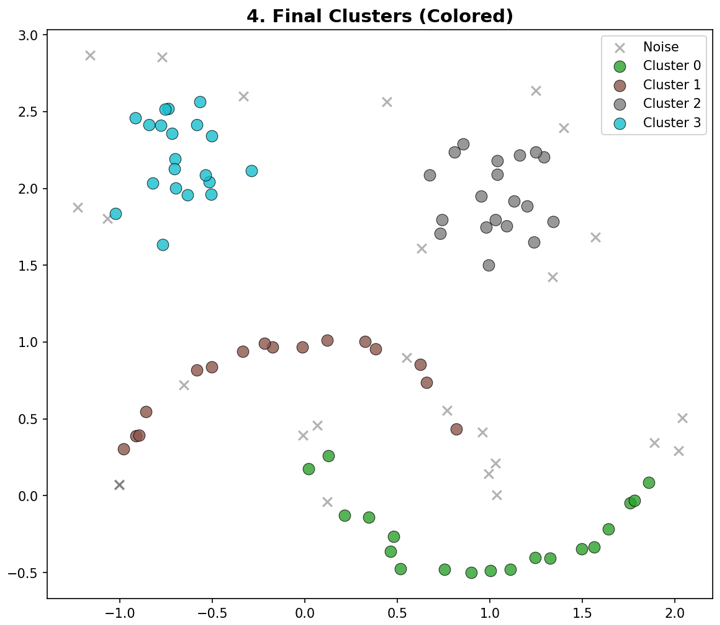
\includegraphics[width=0.5\textwidth]{image/img_7.png}
\caption{Résultat du clustering HDBSCAN sur les données synthétiques (illustration complémentaire).}
\label{fig:results_img_7}
\end{figure}


\section{Comparaison avec DBSCAN}

Le tableau suivant présente une comparaison systématique entre DBSCAN et HDBSCAN :

\begin{table}[htbp]
\centering
\begin{tabular}{lcc}
\toprule
\textbf{Critère} & \textbf{DBSCAN} & \textbf{HDBSCAN} \\
\midrule
Paramètres & $\epsilon$, minPts & minPts, min\_cluster\_size \\
Sélection automatique & Non & Oui (GAP) \\
Densités variables & Non & Oui \\
Clusters non convexes & Oui & Oui \\
Structure hiérarchique & Non & Oui \\
Gestion du bruit & Oui & Oui \\
Complexité & $O(n \log n)$ & $O(n^2)$ à $O(n \log n)$ \\
Sensibilité aux paramètres & Élevée & Faible \\
\bottomrule
\end{tabular}
\caption{Comparaison entre DBSCAN et HDBSCAN.}
\label{tab:comparison}
\end{table}

Les avantages principaux d'HDBSCAN sur DBSCAN sont :
\begin{enumerate}
    \item \textbf{Sélection automatique du seuil} : L'algorithme GAP identifie le seuil optimal sans intervention de l'utilisateur.
    \item \textbf{Robustesse aux densités variables} : La distance d'atteignabilité mutuelle normalise les densités locales.
    \item \textbf{Information hiérarchique} : Le dendrogramme permet une analyse multi-échelle des données.
\end{enumerate}

\section{Conclusion}

Ce rapport a présenté une analyse approfondie de l'algorithme HDBSCAN, en mettant l'accent sur les fondements mathématiques et l'implémentation algorithmique. Les contributions principales d'HDBSCAN sont la transformation des distances par atteignabilité mutuelle, qui permet de gérer des clusters de densités variables, et l'extraction automatique des clusters par l'algorithme GAP ou par maximisation de la stabilité.

\subsection*{Avantages}

HDBSCAN présente plusieurs avantages significatifs pour la pratique du clustering : il nécessite peu de paramétrage grâce à la sélection automatique du seuil, il détecte des clusters de formes arbitraires et de densités hétérogènes, et il fournit une mesure de confiance pour chaque point via la stabilité des clusters.

\subsection*{Limitations}

Les principales limitations concernent la complexité algorithmique, qui peut être prohibitive pour les très grands jeux de données, et la sensibilité au choix du paramètre $min\_pts$ pour les données de très haute dimensionnalité.

\subsection*{Applications}

HDBSCAN trouve des applications dans de nombreux domaines : segmentation d'images médicales, détection d'anomalies en cybersécurité, analyse de données transcriptomiques, et classification d'objets astronomiques. Sa capacité à gérer le bruit et les densités variables en fait un outil privilégié pour l'analyse exploratoire de données complexes.

\section*{Github projet}

Code source du projet : \url{https://github.com/Elorgin29/hdbscan-project}

\nocite{*}
\bibliographystyle{alpha}
\bibliography{bibliography}

\end{document}
